% $File: expr.tex
% $Date: Wed Jan 07 20:05:48 2015 +0800
% $Author: jiakai <jia.kai66@gmail.com>

\section{实验}
关于卷帘快门的参数测量已在\secref{rolling-shutter}中描述,在此不再赘述。
本节中主要介绍前述算法在合成数据和实际数据上的表现情况。

\subsection{基于合成全局快门数据的全局运动分析\label{sec:synth-global}}
% f{{{
使用如下公式合成可控位移的图像,其效果如\figref{synthesis}所示:
\begin{equation}
    f(x, y) = \sin(\omega_x (x + \delta_x)) + \sin(\omega_y y) + 
    \mathcal{N}(0, \sigma^2)
    \label{eqn:synth-global}
\end{equation}
其中$\delta_x$控制位移,$\sigma$控制噪声,$f(x, y)$被量化到$[0, 255]$间的整数。
\begin{figure}[h!]\begin{center}
    \begin{subfigure}[b]{.35\figwidth}
        \centering
        
\includegraphics[width=.35\figwidth]{res/synth0.png}
    \end{subfigure}
    \begin{subfigure}[b]{.35\figwidth}
        \centering
        \includegraphics[width=.35\figwidth]{res/synth1.png}
    \end{subfigure}
    \caption{合成数据,$\delta_x = 0.01$pxl, $\sigma = 1.35/255$}
    \label{fig:synthesis}
\end{center}\end{figure}

控制$\delta_x$取不同的值,按\eqnref{global-phasediff}得到的相位差如
\figref{synthesis:pd}所示。
\begin{figure}[h!]\begin{center}
    \includegraphics[width=.5\figwidth]{res/synth-pd.png}
    \caption{位移与相位差的关系}
    \label{fig:synthesis:pd}
\end{center}\end{figure}

总的来说,基于合成数据的实验证明了前述算法的可行性,
显示相位差与实际位移线性相关,而且对噪声比较鲁棒,
在$\sigma \le 3/255$时都比较有效,已经远低于一般设备的噪声;
但在$\sigma=0$时出现了较大波动,猜测这是由于量化时取整带来的bias造成的,
而在有噪声时可一定程度上抵消这种bias。而为何在噪声太大时由正相关变成了反相关,
我们还没有找到明确的解释。

% f}}}

\subsection{基于实际数据的全局运动分析与低频信号恢复\label{sec:data-global}}
% f{{{

把坐标纸贴在扬声器的震膜上直接拍摄,用扬声器播放10hz, 15hz, 20hz, 25hz的声音,
用Pentax K-01相机拍摄,快门速度为1/2000, iso100, F/5.6, 55mm, 视频为1280x720,
59.940fps, H.264编码。

使用上述方法估计全局运动并直接作为采样信号进行FFT,
发现对单频音和多频音均能较好恢复,
多频音的结果如\figref{real:lowfreq}所示。
\begin{figure}[h!]\begin{center}
    \begin{subfigure}[b]{.5\figwidth}
        \includegraphics[width=.5\figwidth]{res/setting.png}
        \caption{实际拍摄情况}
    \end{subfigure}
    \begin{subfigure}[b]{.5\figwidth}
        \includegraphics[width=.5\figwidth]{res/global-recon.png}
        \caption{重建结果,可见对各频率均能较好恢复;
            其中后半部分的振幅偏高是由于拍摄时误碰了实验装置造成整体位移,
            但对结果影响不大}
    \end{subfigure}
    \caption{基于全局运动分析的低频信号重建}
    \label{fig:real:lowfreq}
\end{center}\end{figure}

% f}}}

\subsection{基于合成卷帘快门数据的局部运动分析,
    及基于MSA算法的高频信号恢复\label{sec:synth-local}}
% f{{{
与\secref{synth-global}类似,我们先用合成数据的方法测试算法的可行性。
对\eqnref{synth-global}进行修改,我们使用如下方法合成一段视频,对于第$i$帧:
\begin{eqnarray}
    f(i, x, y) &=& \sin(\omega_x (x + \delta_x(i, y))) + \sin(\omega_y y) + 
    \mathcal{N}(0, \sigma^2) \\
    \delta_x(i, y) &=& A\sin(2\pi f_s(it_f+yd))
    \label{eqn:synth-local}
\end{eqnarray}
实验中,在\eqnref{synth-local}里我们取$A=0.01$表示震动造成的水平位移为$0.01$像素,
$t_f=\frac{1}{60}$为视频每帧的时长,$d=1.57e-5$为线延迟,$f_s=500$为震动频率,
另外$f(i, x, y)$量化到$[0, 255]$间的整数并加上方差为1的白噪声。
另外我们还选取了$f_s=\{500, 800\},\,A=\{0.01, 0.005\}$进行多频音的测试。
对视频前10帧用\secref{algo-hf}所述的方法进行频谱恢复,
结果如\figref{synth-local}所示,
可见在噪声存在的情况下,
该方法能较为准确的恢复卷帘快门成像所包含的高频运动信息。
\begin{figure}[h!]\begin{center}
    \begin{subfigure}[b]{.5\figwidth}
        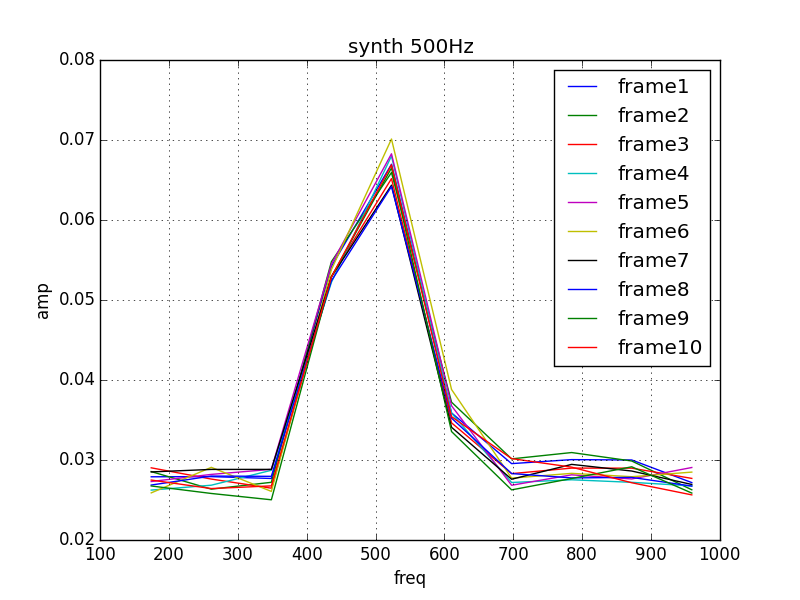
\includegraphics[width=.5\figwidth]{res/synth-500.png}
        \caption{500Hz合成数据的恢复}
    \end{subfigure}
    \begin{subfigure}[b]{.5\figwidth}
        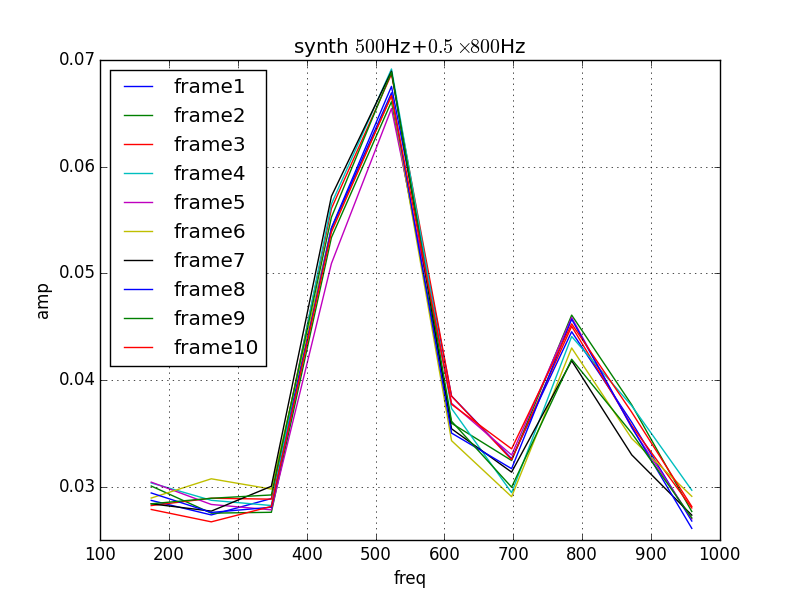
\includegraphics[width=.5\figwidth]{res/synth-500+800.png}
        \caption{500Hz和800Hz,振幅$2:1$合成数据的恢复}
        \label{fig:synth:500+800}
    \end{subfigure}
    \caption{对合成的卷帘快门视频进行频谱分析的结果}
    \label{fig:synth-local}
\end{center}\end{figure}
% f}}}

\subsection{MSA算法的合理性及其中参数的选择}
% f{{{
MSA算法中两个比较重要的参数是$\theta_m$和$g_\theta$,
分别控制图像金字塔的高度和按列分组平均的组大小。
在这里我们用实验方法确定其取值,同时也说明MSA算法的合理性。

我们采用从实际拍摄数据(见\secref{data-local})重建的频谱的信噪比
作为性能评价指标。我们已知真实数据是单频音,
因此把频谱中能量最强的频率作为信号,其余作为噪声,并随机取了
3幅参考帧和3幅目标帧,计算9次重建的平均信噪比。
调整$\theta_m$和$g_\theta$,可以得到以下数据:
\begin{figure}[h!]\begin{center}
    \begin{subfigure}[b]{.33\figwidth}
        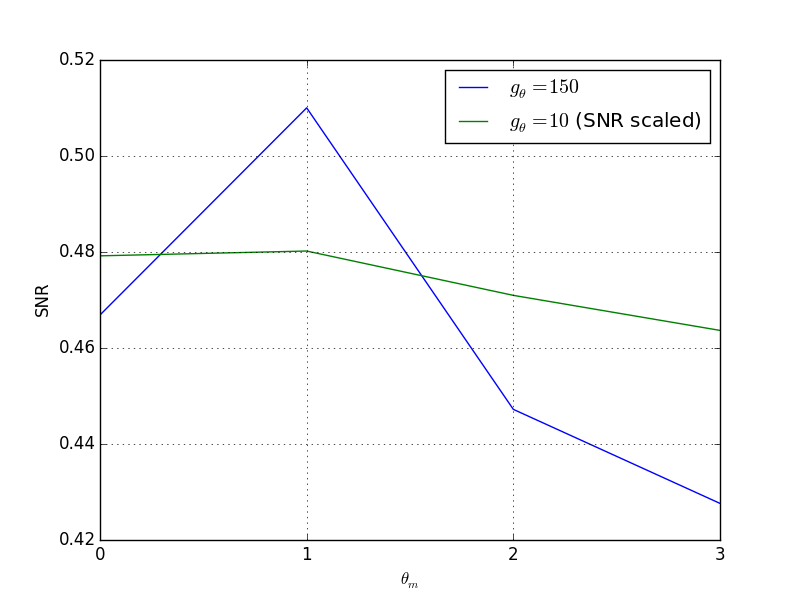
\includegraphics[width=.33\figwidth]{res/msa-lvl.png}
        \caption{SNR与$\theta_m$的关系}
        \label{fig:msa:lvl}
    \end{subfigure}
    \begin{subfigure}[b]{.33\figwidth}
        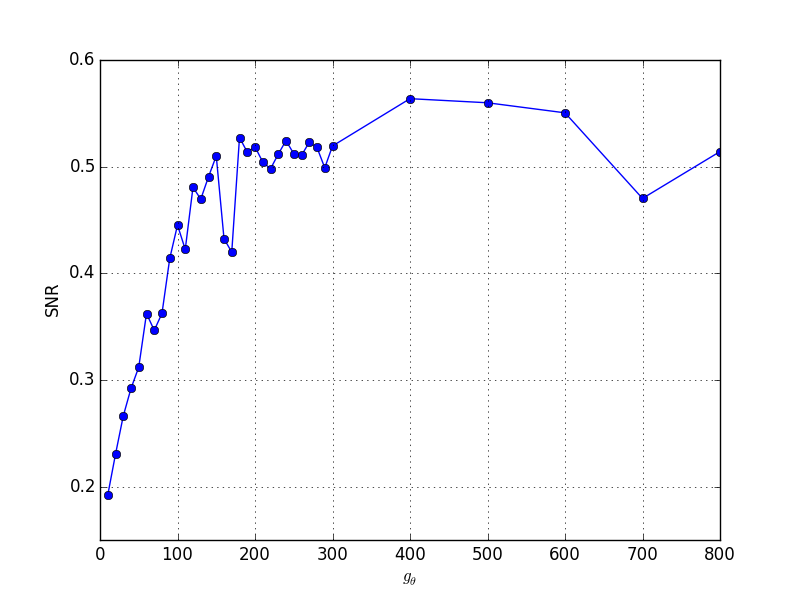
\includegraphics[width=.33\figwidth]{res/msa-vg.png}
        \caption{SNR与$g_\theta$的关系}
        \label{fig:msa:vg}
    \end{subfigure}
    \begin{subfigure}[b]{.33\figwidth}
        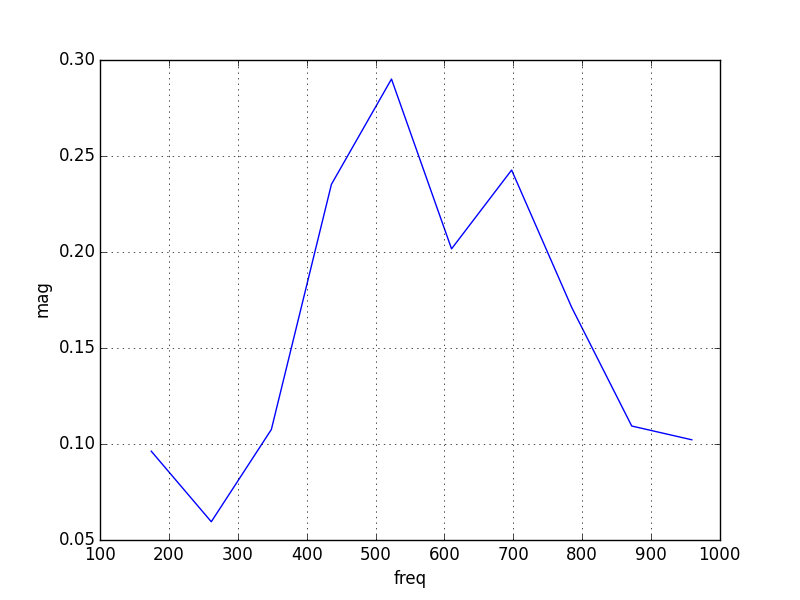
\includegraphics[width=.33\figwidth]{res/msa-800.png}
        \caption{$g_\theta$太大时的实际重建频谱}
        \label{fig:msa:800}
    \end{subfigure}
    \caption{MSA调参情况}
    \label{fig:msa}
\end{center}\end{figure}

从这些数据中有以下发现:
\begin{enumerate}
    \item \figref{msa:lvl}说明MSA中取多个尺度求平均是可以提高性能的,
        具体而言在$\theta_m=1$,即取两个尺度时性能较好;同时也说明了
        $g_\theta$和$\theta_m$对SNR的影响基本正交。
    \item 在\figref{msa:vg}中看似$g_\theta$越大越好,
        但观察在其取值较大时的实际重建频谱\figref{msa:800}可发现,
        尽管SNR比较高,却出现了两个尖峰,是很严重的artifact。
        因此一方面SNR并不是评价性能的最好指标,
        另一方面MSA中按列分组取平均也是可提高鲁棒性的。
        我们观察发现,整体而言$g_\theta$越大,
        频谱越有变宽或者出现多个尖峰的趋势,
        最终我们取了$g_\theta=150$作为比较折衷的值。
\end{enumerate}

另外,我们也尝试了对多个尺度取不同的$g_\theta$,具体而言令
$g_\theta=\frac{150}{2^\theta}$,发现SNR从0.51降至0.40,
因此最终选择了常数的$g_\theta=150$。
% f}}}

\subsection{基于实际数据和MSA算法的局部运动分析与高频信号恢复
    \label{sec:data-local}}
% f{{{
与\secref{data-global}采用相同的相机配置,如\secref{algo-hf}所述取
$\theta_m=1$,此时采样率上限为
$\frac{1}{d2^{\theta_m}} \approx 27000$Hz,
而实际可用的采样频率还受限于快门速度,大概不超过$1000$Hz。

我们对单频和双频音进行了测试,发现单频音恢复效果总体不错,
但双频音则效果很差。具体如\figref{real:highfreq}所示。
\begin{figure}[h!]\begin{center}
    \begin{subfigure}[b]{.33\figwidth}
        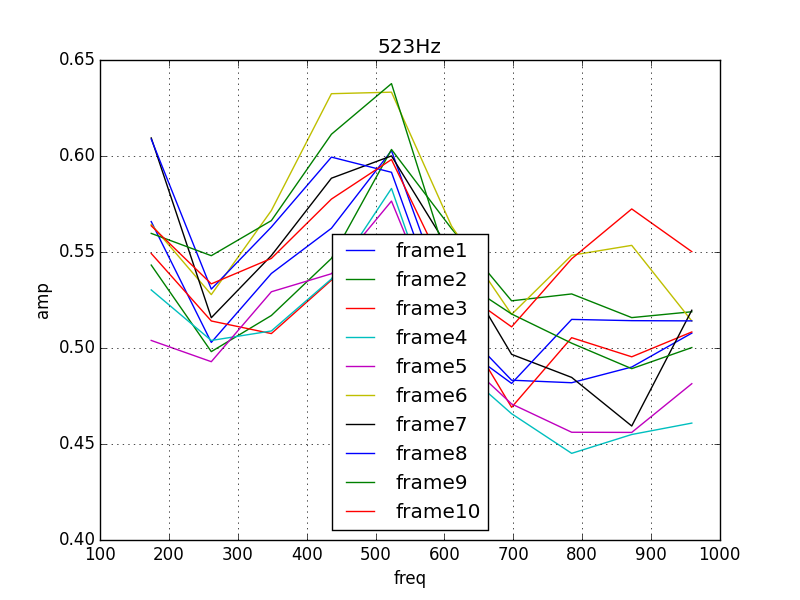
\includegraphics[width=.33\figwidth]{res/data-523.png}
        \caption{$\text{C}_5$(523Hz)单频音的恢复}
    \end{subfigure}
    \begin{subfigure}[b]{.33\figwidth}
        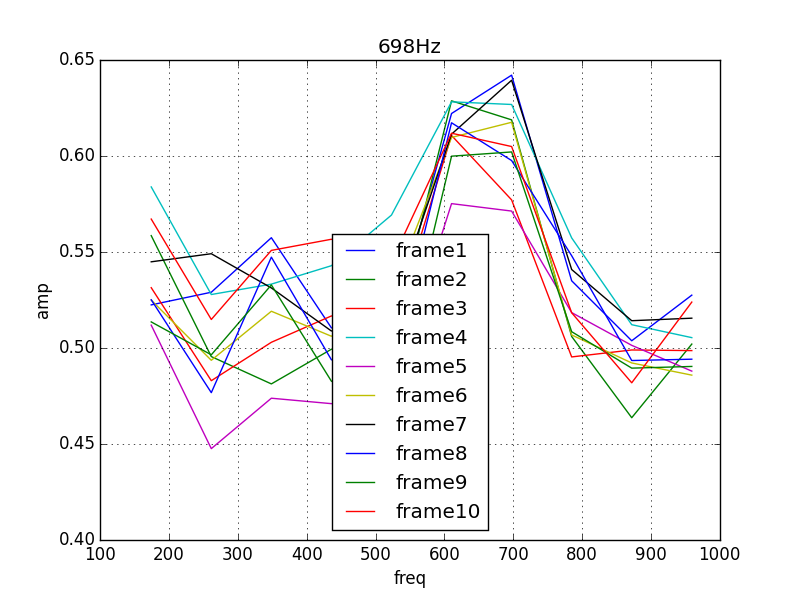
\includegraphics[width=.33\figwidth]{res/data-698.png}
        \caption{$\text{F}_5$(698Hz)单频音的恢复}
    \end{subfigure}
    \begin{subfigure}[b]{.33\figwidth}
        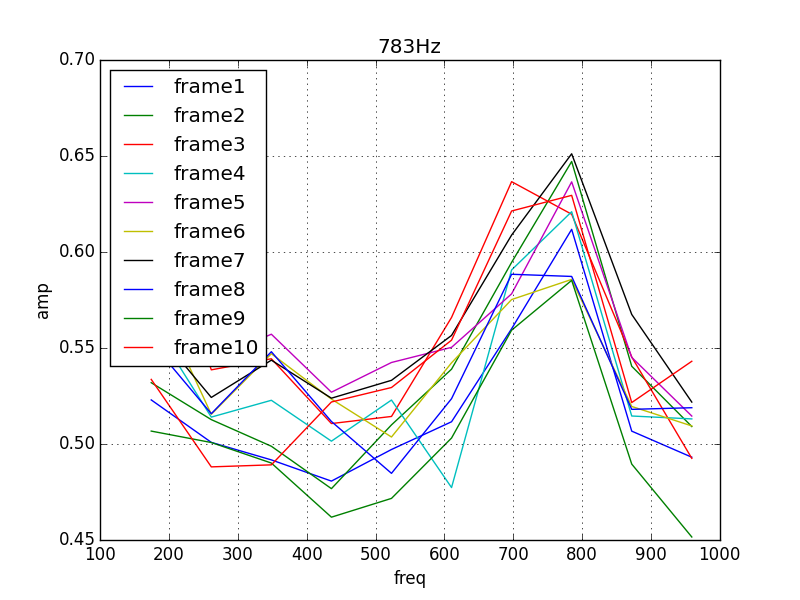
\includegraphics[width=.33\figwidth]{res/data-783.png}
        \caption{$\text{G}_5$(783Hz)单频音的恢复}
    \end{subfigure}
    \begin{subfigure}[b]{.4\figwidth}
        \includegraphics[width=.4\figwidth]{res/data-300+500.png}
        \caption{等幅300Hz+500Hz双频音的恢复}
        \label{fig:real:300+500}
    \end{subfigure}
    \begin{subfigure}[b]{.4\figwidth}
        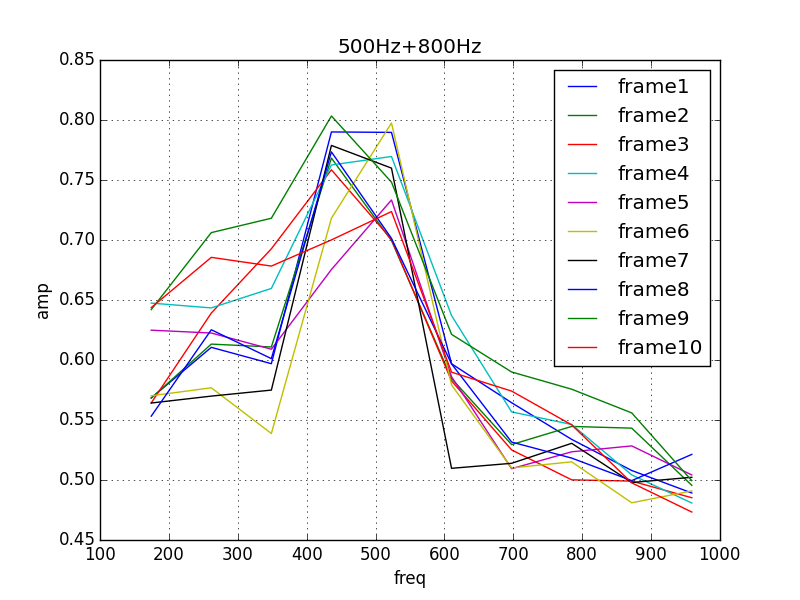
\includegraphics[width=.4\figwidth]{res/data-500+800.png}
        \caption{等幅500Hz+800Hz双频音的恢复}
    \end{subfigure}
    \caption{对实际拍摄视频进行频谱分析的结果}
    \label{fig:real:highfreq}
\end{center}\end{figure}
% f}}}

\subsection{全局优化}
% f{{{
全局优化分为频谱的指数插值和G\&L迭代两步,已在\secref{global-opt}中详述。
在这里我们展示优化过程中信号的变化情况,如\figref{global-opt}所示。
可以观察到随着迭代的进行,信号逐渐变得平滑。在大约200次迭代后,
就能得到比较稳定的解,播放后人耳可以辨认出单频音的音高。
相关视频和音频在本文的补充材料中。
\begin{figure}[h!]\begin{center}
    \begin{subfigure}[b]{\figwidth}
        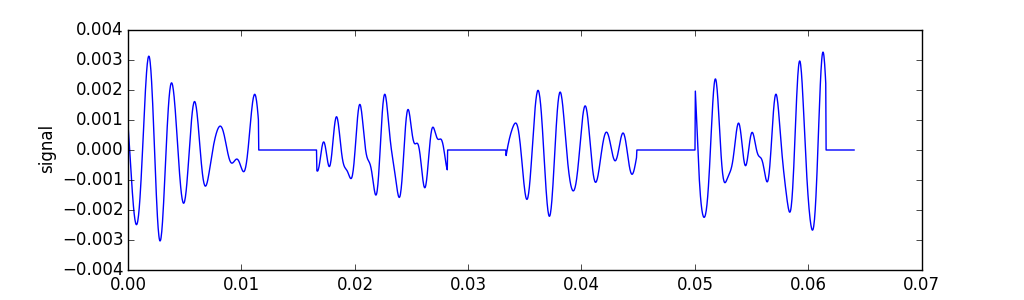
\includegraphics[width=\figwidth]{res/opt00.png}
        \caption{全局优化的初始解}
    \end{subfigure}
    \begin{subfigure}[b]{\figwidth}
        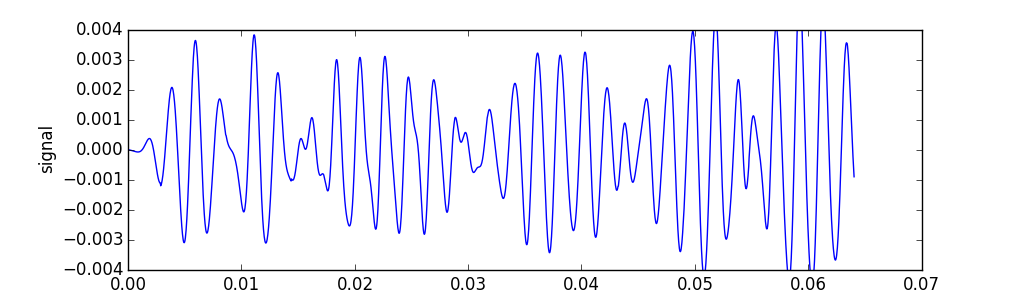
\includegraphics[width=\figwidth]{res/opt01.png}
        \caption{迭代1步后的情况}
    \end{subfigure}
    \begin{subfigure}[b]{\figwidth}
        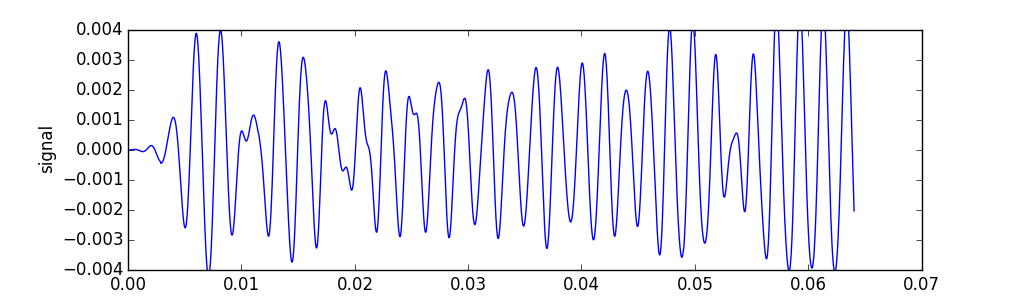
\includegraphics[width=\figwidth]{res/opt20.png}
        \caption{迭代20步后的情况}
    \end{subfigure}
    \begin{subfigure}[b]{\figwidth}
        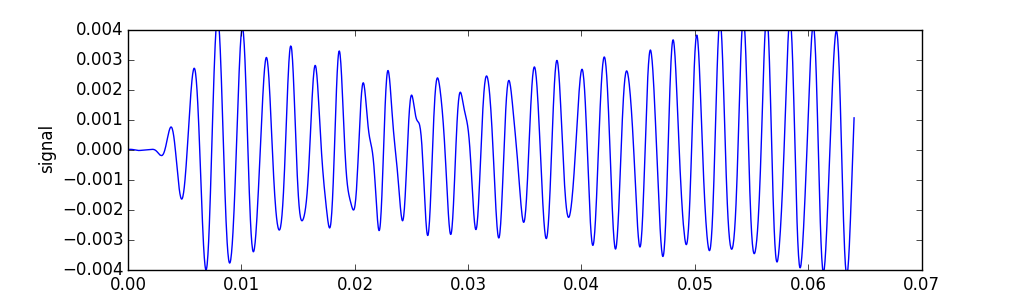
\includegraphics[width=\figwidth]{res/opt200.png}
        \caption{迭代200步后的情况}
    \end{subfigure}
    \caption{全局优化过程}
    \label{fig:global-opt}
\end{center}\end{figure}
% f}}}

% vim: filetype=tex foldmethod=marker foldmarker=f{{{,f}}} 
